% This must be in the first 5 lines to tell arXiv to use pdfLaTeX, which is strongly recommended.
\pdfoutput=1
% In particular, the hyperref package requires pdfLaTeX in order to break URLs across lines.

\documentclass[11pt]{article}

% Remove the "review" option to generate the final version.
\usepackage[review]{ACL2023}
% \usepackage{ACL2023}

% Standard package includes
\usepackage{times}
\usepackage{latexsym}
\usepackage{tipa}
\usepackage{subfiles}
\usepackage{booktabs}                         % better-looking tables
\usepackage[raggedrightboxes]{ragged2e}       % better table alignment
\usepackage{subfiles}                         % file management
\usepackage{longtable}                        % multi-column tables
\usepackage{amsmath}                          % math symbols and equations
\usepackage{graphicx}                         % inserting images

% For proper rendering and hyphenation of words containing Latin characters (including in bib files)
\usepackage[T1]{fontenc}
% For Vietnamese characters
% \usepackage[T5]{fontenc}
% See https://www.latex-project.org/help/documentation/encguide.pdf for other character sets

% This assumes your files are encoded as UTF8
\usepackage[utf8]{inputenc}

% This is not strictly necessary, and may be commented out.
% However, it will improve the layout of the manuscript,
% and will typically save some space.
\usepackage{microtype}

% This is also not strictly necessary, and may be commented out.
% However, it will improve the aesthetics of text in
% the typewriter font.
\usepackage{inconsolata}

\title{Developing a Named Entity Recognition Dataset for Tagalog}

\author{Lester James V. Miranda \\
  \texttt{ljvmiranda@gmail.com} \\}

\begin{document}
\newcommand{\tlunified}{\textsc{TLUnified-NER}}

\maketitle
\begin{abstract}
  We present the development of a Named Entity Recognition (NER) dataset for Tagalog.
  This corpus helps fill the resource gap present in Philippine languages today, where NER resources are scarce.
  The texts were obtained from a pretraining corpora containing news reports, and were labeled by native speakers in an iterative fashion.
  The resulting dataset contains $\sim$7.8k documents across three entity types: Person, Organization, and Location.
  The inter-annotator agreement, as measured by Cohen's $\kappa$, is 0.81.
  We also conducted extensive empirical evaluation of state-of-the-art methods across supervised and transfer learning settings.
  Finally, we released the data and processing code publicly to inspire future work on Tagalog NLP.
\end{abstract}

\section{Introduction}

Tagalog (\texttt{tl}) is one of the major languages in the Philippines with over 28 million speakers in the country \cite{Lewis2009EthnologueL}. 
It constitutes the bulk of Filipino, the country's official language, by sharing its lexical items and grammatical structure.
Despite this fact, there are little to no resources for Tagalog \cite{Cruz2021ImprovingLL}, hampering the development of reliable language technologies.

In this paper, we present \tlunified{},\footnote[1]{The dataset is accessible at \url{https://osf.io/da37u/?view_only=e134831fe07749918c9188b5b4715f1f}} a Tagalog dataset for Named Entity Recognition (NER).
The texts were obtained from TLUnified \cite{Cruz2021ImprovingLL}, a pretraining corpora containing news reports and other types of text.
We focused on NER because of its foundational role in several NLP tasks \citep{Sang2003IntroductionTT,Lample2016NeuralAF}, especially in problems that require the extraction of structured information. 
\tlunified{} consists of $\sim$7.8k documents across three entity types (\textit{Person}, \textit{Organization}, \textit{Location}), modeled closely to the CoNLL Shared Tasks \cite{Sang2002IntroductionTT,Sang2003IntroductionTT}.
Three native speakers conducted the annotation process, resulting to an inter-annotator agreement (IAA) score of 0.81.

We hope that \tlunified{} will allow researchers to build better NER classifiers for Tagalog, and thereby inspire future research on Tagalog NLP through the following contributions:

\begin{enumerate}
  \item We curated and annotated texts from a large pretraining corpora to represent the modern usage of Tagalog in the news domain.
  \item We provided performance baselines across a variety of supervised and transfer learning settings.
\end{enumerate}

\section{Related Work}


\subfile{tables/entity_types}

\paragraph{Tagalog language} 
Tagalog is an agglutinative language within the Austronesian family \cite{Kroeger1992PhraseSA}. 
It uses the Latin script for its writing system with 28 letters in its alphabet. 
Twenty-six letters are the same as in English, with the addition of \~{N}/\~{n} and Ng/ng.
Tagalog typically follows the VSO word order, but VOS and SVO are also accepted \citep{Schachter1973TagalogRG}.
Although Filipino is the country's official language, it has little to no linguistic differences with Tagalog.

\paragraph{Tagalog NER datasets}
Unfortunately, resources for Tagalog NER are meager.
One major resource is WikiANN \cite{Pan2017CrosslingualNT}, a silver-standard corpora based on a framework designed for 282 other languages.  
However, the Tagalog portion of WikiANN is full of annotation errors, often misconstruing one entity type as another.
Another NER dataset is the Filipino Storytelling corpora \cite{Costiniano2022CustomCG}. 
Although gold-standard, its entity labels (e.g., \textit{Humans \& Body}, \textit{Natural Environment}, etc.) are too domain-specific for general use.
Finally, the LORELEI project also provides language packs for Tagalog \cite{Strassel2016LORELEILP}, but they're not publicly-accessible.

\tlunified{} aims to fill this resource gap by providing a publicly-assessible gold standard resource for Tagalog NER.


\section{Dataset Collection}

The texts were obtained from \citet{Cruz2021ImprovingLL}'s TLUnified pretraining corpora.
It combines news reports \citep{Cruz2020ExploitingNA}, a preprocessed version of CommonCrawl \citep{OrtizSuarez2019AsynchronousPF}, and several other datasets.
We manually filtered this dataset to contain news reports so as to resemble the CoNLL Shared Tasks \cite{Sang2002IntroductionTT,Sang2003IntroductionTT}.

The texts are diverse. 
It contains articles from different news sites online that ran a published print media or news channel in Metro Manila from 2009 to early 2020.
The topics range from politics, weather, and popular science among others.

\section{Annotation Setup}

We used Prodigy as our annotation tool.\footnote[2]{\url{https://prodigy.ai}}
We set up a web server on the Google Cloud Platform and routed the examples through Prodigy's built-in task router.
Figure \ref{fig:annotation_interface} shows the labeling interface as seen by the annotator.
Finally, we used the \texttt{ner.manual} recipe to highlight spans during the annotation process.
We used three entity labels for \tlunified{} as shown in Table \ref{table:entity_types}.
Unlike CoNLL, we decided to exclude the \textit{Miscellaneous (MISC)} tag to reduce confusion.

\subfile{tables/dataset_statistics.tex}

\begin{figure}[t]
\frame{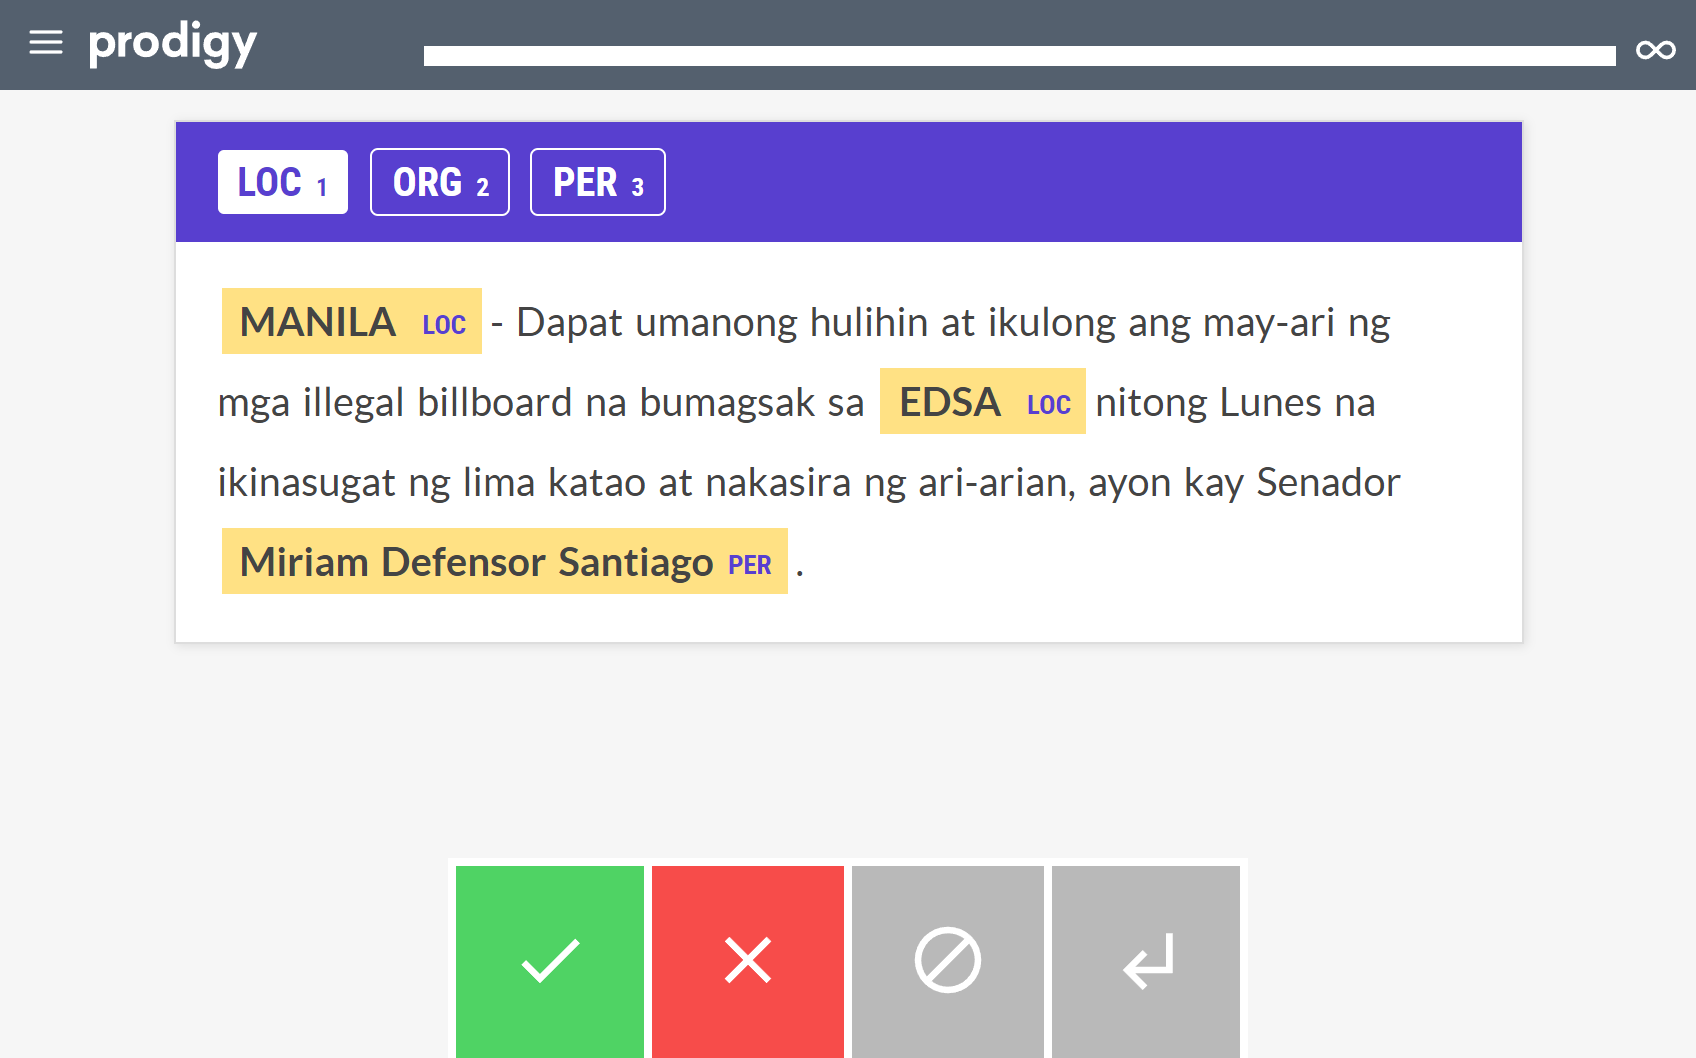
\includegraphics[width=0.48\textwidth]{figures/annotation_interface.png}}
\caption{
  Prodigy's annotation interface for a given text. 
  (Translation: \textit{MANILA - The owner of the illegal billboards that fell on EDSA this Monday, injuring five people and damaging property, should be caught and imprisoned according to Senator Miriam Defensor Santiago.})
}
\label{fig:annotation_interface}
\centering
\end{figure}


\paragraph{Annotation Process}
The annotation process was done iteratively with three annotators (including the author) who are native Tagalog speakers.
Given a set annotation budget, we paid the annotators above the country's minimum daily wage.
Each annotation round spans for two to three weeks, for a total of six rounds (18 weeks).
The annotators labeled the same batch of examples to ensure high overlap.

After each round, the annotators hold a retrospective meeting and discussed examples they found confusing, inconsistent with the annotation guidelines, and noteworthy.
This process continued until we reached $\sim$10k examples or if we exhausted our annotation budget.
In addition, we also tracked the training curve to determine the quality of the collected annotations.
If the F1-score improved within the last 25\% of the training data, then it is a good sign that obtaining more labels will result to better accuracy.

\paragraph{Annotation Guidelines}
We developed the annotation guidelines in an iterative fashion. 
The Automatic Content Extraction (ACE 2004/05) annotation document \cite{Doddington2004TheAC} heavily inspired our initial draft.
We co-developed the guidelines after each annotation round to improve clarity and reduce disagreements.
These guidelines are accessible on GitHub: \url{https://anonymous.4open.science/r/tagalog-ner-B902/datasets/tl_XXXX-1_gold_corpus/guidelines/README.md}

\section{Corpus Statistics and Evaluation}

Table \ref{table:dset_stats} shows the final dataset statistics for \tlunified{}.
We also included span- (SD) and boundary-distinctiveness (BD) metrics \cite{Papay2020DissectingSI}.
They measure the KL-divergence of the unigram word distributions between the span (or its boundaries) and the rest of the corpora.
These metrics can be used to gauge the difficulty of the span labeling task, (e.g., more distinct spans means it's ``easier'' to detect them in the text). 

\subfile{tables/iaa}


\subsection{Inter-annotator Agreement (IAA)}

Similar to \citet{Brandsen2020CreatingAD}, we measured two types of Cohen's $\kappa$. 
The first metric calculates $\kappa$ for tokens where at least one annotator has made an annotation. 
The second metric computes for all tokens while ignoring the `O' label.
In addition, we had a third measure: the F1-score using one set of annotations as reference \cite{Deleger2012BG}.
We did these computations for each annotator-pair and averaged the results as shown in Table \ref{table:iaa}.

Finally, Figure \ref{fig:iaa} shows the growth of IAA for each annotation round.
Because of our annotation process, we were able to label the same batch of documents and track the agreement every round.


\begin{figure}[t]
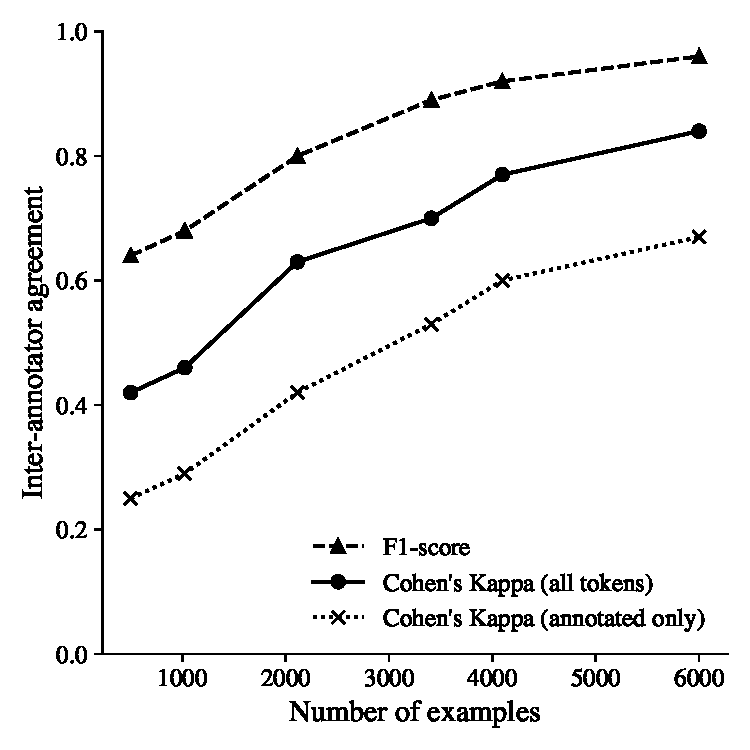
\includegraphics[width=0.5\textwidth]{figures/iaa}
\caption{Growth of IAA for each annotation round.}
\label{fig:iaa}
\centering
\end{figure}


\subsection{Benchmark results}


\subfile{tables/results_baseline}

We trained several NER models using spaCy's transition-based parser \cite{Honnibal2020Spacy}.
The state transitions are based on the BILUO sequence encoding scheme and the actions are decided by a convolutional neural network with a maxout \cite{Goodfellow2013MaxoutN} activation function.

While keeping the NER classifier constant, we experimented with various word embeddings that led to the following configurations:

\begin{itemize}
  \item \textbf{Baseline:} we trained the transition-based parser ``from scratch'' without additional information from static or context-sensitive vectors.
  \item \textbf{Static vectors:} we used Tagalog fastText vectors \cite{Bojanowski2016EnrichingWV} and included a simple pretraining process to initialize the weights of the model.
  The pretraining objective asks the model to predict some number of leading and trailing UTF-8 bytes for the words\textemdash a variant of the cloze task.
  \item \textbf{Transformer-based vectors (monolingual):} we used RoBERTa Tagalog \cite{Cruz2021ImprovingLL}, the only pretrained language model for Tagalog, and finetuned it with our annotations.
  \item \textbf{Transformer-based vectors (multilingual):} we tested on XLM-RoBERTa \cite{Conneau2019UnsupervisedCR} and multilingual BERT \cite{Devlin2019BERTPO} for transfer learning.
  These models include Tagalog in their training pool albeit underrepresented.
\end{itemize}

This experimental setup allows us to see the expected performance when training Tagalog NER classifiers using standard techniques.
Table \ref{table:results_baseline} reports the F1-score on the test set across three trials.


\begin{figure}[t]
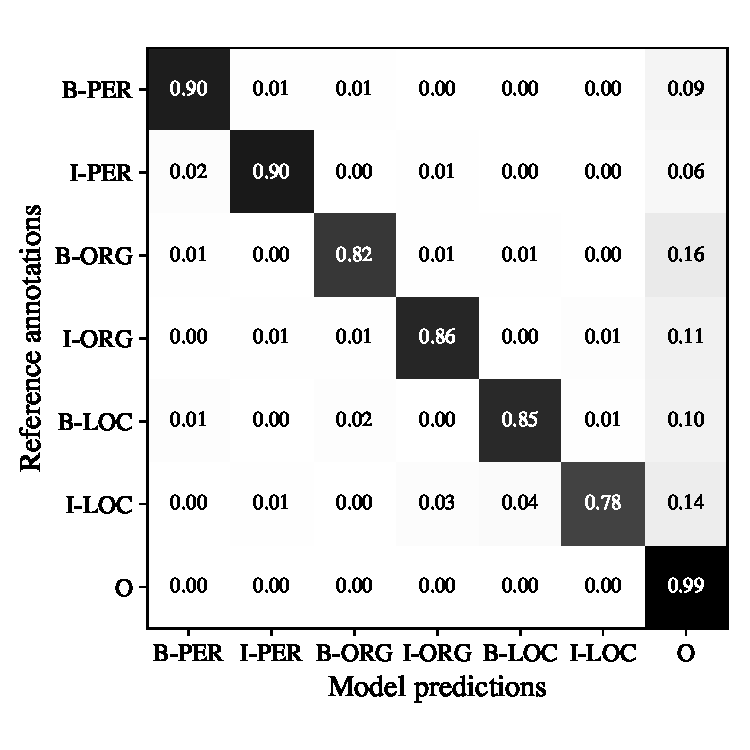
\includegraphics[width=0.5\textwidth]{figures/confusion}
\caption{Development set confusion matrix of the Baseline model predictions in the IOB format.}
\label{fig:confusion}
\centering
\end{figure}

\subsection{Error analysis}

From our benchmark results, we noticed that most models are having trouble predicting the \textit{Location} or \textit{Organization} tags.
Figure \ref{fig:confusion} shows the confusion matrix of the Baseline model on the development set in the IOB format.

Most of the mistakes came from incorrectly tagging a token with the outside `O' label.
However, we also noticed instances where the model confuses between the lexical and semantic tag of an entity.
For example, in the span, \textit{``..panukala ng Ombudsman...''} (``...proposed by the Ombudsman...''), the token \texttt{Ombudsman} might be a Person or Organization depending on the context.
Using context-sensitive vectors helped mitigate this issue.

Given the IAA and benchmark results, we posit that \tlunified{} is a learnable task.
We encourage researchers to utilize context-sensitive vectors when training models from this corpora.


\section{Conclusion}

In this paper, we introduced \tlunified{}, a Named Entity Recognition dataset for Tagalog.
Unlike other Tagalog NER datasets, \tlunified{} is publicly-accessible and gold standard.
Our iterative annotation process, together with our inter-annotator agreement, shows that the corpus is of high quality.
In addition, our benchmarking results suggest that the task is learnable even with a simple baseline method.

We hope that \tlunified{} fills the resource gap present in Tagalog NLP today.
In the future, we plan to create a more fine-grained (and perhaps, overlapping) NER tag set similar to the ACE project and expand on other major Philippine languages.
Finally, the dataset is available online (\url{https://osf.io/da37u/?view_only=e134831fe07749918c9188b5b4715f1f}) and we encourage researchers to improve upon our benchmark results.


\section*{Limitations}

The \tlunified{} corpora is comprised mostly by news reports.
Although the texts demonstrate the standard usage of Tagalog, its domain is limited.
In addition, we only trained a transition-based parser model for our NER classifier.
In the future, we plan to extend these benchmarks and include CRFs or other tools such as Stanford Stanza.


\bibliography{custom}
\bibliographystyle{acl_natbib}


\end{document}
